% Week 1 — Lecture: Introduction to Git and GitHub
% Course: Model-Based Decisions (2025)
% MSc Computational Science, University of Amsterdam
% Uses Arguelles Beamer Theme

\documentclass[aspectratio=169,13pt]{beamer}
\usetheme{Arguelles}

\usepackage{fontspec}
\usepackage{unicode-math}
\usepackage{graphicx}
\usepackage{tikz}


\usetikzlibrary{positioning, arrows.meta}
\usepackage{minted}
\setminted{fontsize=\scriptsize, bgcolor=gray!5, frame=single}

\title{Introduction to Git and GitHub}
\subtitle{Model-Based Decisions — Week 1 Practical}
\author{Michael Lees}
\institute{Computational Science Lab, University of Amsterdam}
\date{October 2025}

\begin{document}

\begin{frame}
    \titlepage
\end{frame}

% -------------------------------------------------------------
\begin{frame}{Motivation: Why Version Control?}
    \begin{itemize}
        \item Research and code evolve — we need a record of changes over time.
        \item Collaboration: work safely with others without overwriting each other's files.
        \item Reproducibility: recover previous versions and ensure results can be traced.
        \item Backup: your work is stored remotely (e.g., on GitHub) as well as locally.
    \end{itemize}
    \pause
    \vspace{1em}
    \begin{block}{Without version control}
        \texttt{final\_report\_v2\_fixed\_final\_FINAL.docx}
    \end{block}
\end{frame}

% -------------------------------------------------------------
\begin{frame}{What is Git?}
    \begin{itemize}
        \item \textbf{Git} is a distributed version control system.
        \item It records snapshots (“commits”) of your project over time.
        \item Every developer has a complete copy of the repository — no central lock-in.
    \end{itemize}
    \vspace{1em}
    \begin{center}
        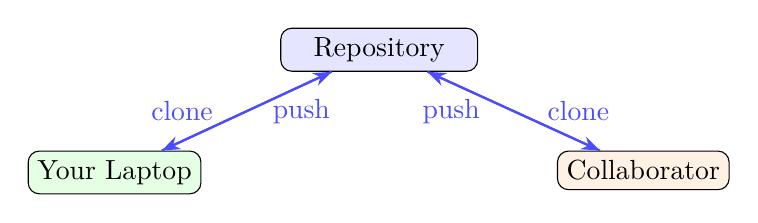
\begin{tikzpicture}[node distance=2.5cm, >=Stealth]
            \node[draw, fill=blue!10, rounded corners, minimum width=2.5cm] (repo) {Repository};
            \node[draw, fill=green!10, rounded corners, below left=1cm and 1cm of repo] (local1) {Your Laptop};
            \node[draw, fill=orange!10, rounded corners, below right=1cm and 1cm of repo] (local2) {Collaborator};

            % shifted label positions
            \draw[->, thick, blue!70] (repo) -- (local1)
            node[midway, left=0.1cm, xshift=-0.2cm] {clone};
            \draw[->, thick, blue!70] (local1) -- (repo)
            node[midway, right=0cm, xshift=0.2cm] {push};

            \draw[->, thick, blue!70] (repo) -- (local2)
            node[midway, right=0.1cm, xshift=0.2cm] {clone};
            \draw[->, thick, blue!70] (local2) -- (repo)
            node[midway, left=0.1cm, xshift=-0.2cm] {push};
        \end{tikzpicture}
    \end{center}
\end{frame}

% -------------------------------------------------------------
\begin{frame}{Key Concepts or Terms}
    \begin{description}[leftmargin=4cm, labelwidth=3cm]
        \item[Repository (repo)] A project folder tracked by Git.
        \item[Commit] A snapshot of your project at a specific point in time.
        \item[Branch] A line of development (default is \texttt{main}).
        \item[Remote] A copy of the repo hosted elsewhere (e.g., GitHub).
        \item[Clone / Push / Pull] Commands to sync local and remote copies.
    \end{description}
\end{frame}

% -------------------------------------------------------------
\begin{frame}[fragile]{Creating and Initializing a Repository}
    \textbf{Step 1: Create a new folder for your project}
    \begin{minted}{bash}
  mkdir my_project
  cd my_project
  \end{minted}

    \textbf{Step 2: Initialize Git}
    \begin{minted}{bash}
  git init
  \end{minted}

    This creates a hidden folder \texttt{.git/} that stores all version history.

    \textbf{Step 3: Check status}
    \begin{minted}{bash}
  git status
  \end{minted}

    This creates a repository \textbf {locally}, on your machine only.
\end{frame}

% -------------------------------------------------------------
\begin{frame}[fragile]{Tracking and Committing Changes}
    \begin{minted}{bash}
  git add my_notebook.ipynb
  git commit -m "Initial commit: added notebook"
  \end{minted}

    \begin{itemize}
        \item \texttt{git add}: This adds the file \texttt{my\_notebook.ipynb} to the staging area. The staging area is where you put changes and new files that you want to include in the next commit.
        \item \texttt{git commit}: permanently records the snapshot with a message specified after \texttt{-m}. This message should describe the changes made in this commit.
    \end{itemize}

    \vspace{0.5em}
    Good commit messages:
    \begin{itemize}
        \item “Added visualization for cellular automaton”
        \item “Fixed bug in update rule”
    \end{itemize}
\end{frame}

% -------------------------------------------------------------
\begin{frame}[fragile]{Connecting to GitHub}
    \begin{enumerate}
        \item Create a free account at \href{https://github.com}{github.com}.
        \item On GitHub: “New Repository” → copy the HTTPS link.
        \item In your terminal:
              \begin{minted}{bash}
    git remote add origin https://github.com/username/my_project.git
    git branch -M main
    git push -u origin main
    \end{minted}
        \item You can now push updates with:
              \begin{minted}{bash}
    git push
    \end{minted}
    \end{enumerate}
\end{frame}

% -------------------------------------------------------------
\begin{frame}{The Basic Git Workflow}
    \begin{center}
        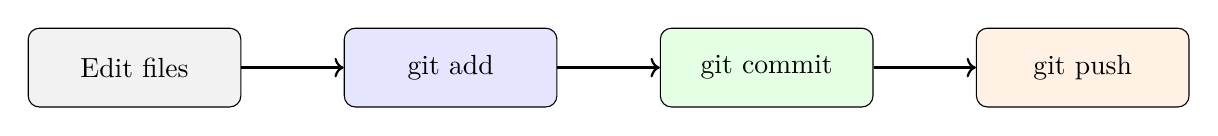
\begin{tikzpicture}[node distance=1.3cm, every node/.style={align=center, rounded corners, minimum width=2.7cm, minimum height=1cm}]
            \node[fill=gray!10, draw] (edit) {Edit files};
            \node[fill=blue!10, draw, right=of edit] (add) {git add};
            \node[fill=green!10, draw, right=of add] (commit) {git commit};
            \node[fill=orange!10, draw, right=of commit] (push) {git push};

            \draw[->, thick] (edit) -- (add);
            \draw[->, thick] (add) -- (commit);
            \draw[->, thick] (commit) -- (push);
        \end{tikzpicture}
    \end{center}

    \vspace{1em}
    \begin{block}{In short}
        \texttt{Edit → Add → Commit → Push}
    \end{block}
\end{frame}

% -------------------------------------------------------------
\begin{frame}[fragile]{Getting Updates from GitHub}
    If others have updated the remote repository (i.e., on GitHub), use:
    \begin{minted}{bash}
  git pull
  \end{minted}
    This downloads and merges changes from the remote repository.

    \vspace{0.5em}
    \begin{itemize}
        \item Always \texttt{pull} before starting new work.
        \item Resolve any merge conflicts carefully — Git will mark conflicting lines.
    \end{itemize}
\end{frame}

% -------------------------------------------------------------
\begin{frame}{Graphical Interfaces (Optional)}
    You do \emph{not} need to use Git only via terminal — several excellent GUI tools exist:

    \begin{itemize}
        \item \textbf{GitHub Desktop} — free, simple interface for beginners
              \url{https://desktop.github.com}
        \item \textbf{VS Code} — built-in Git integration (source control tab).
        \item \textbf{Sourcetree} — Atlassian’s free visual Git client.
    \end{itemize}

    \vspace{0.5em}
    All of these show:
    \begin{itemize}
        \item File differences before committing.
        \item Commit history and branches visually.
        \item Push/pull buttons instead of typing commands.
    \end{itemize}
\end{frame}

% -------------------------------------------------------------
\begin{frame}{Common Pitfalls and Tips}
    \begin{itemize}
        \item Remember to \texttt{git add} before committing — otherwise changes aren’t saved.
        \item Never commit large data files or secrets (API keys, passwords).
        \item Use \texttt{.gitignore} to exclude unnecessary files (e.g., \texttt{.ipynb\_checkpoints/}).
        \item Write descriptive commit messages — your future self will thank you.
    \end{itemize}
\end{frame}

% -------------------------------------------------------------
\begin{frame}{Summary}
    \begin{itemize}
        \item Git keeps a history of your work — like a time machine for your code.
        \item GitHub lets you share and collaborate safely.
        \item Learn the core cycle: \texttt{add → commit → push → pull}.
        \item Use GUI tools if you prefer a visual workflow.
    \end{itemize}

    \vspace{1em}
    \begin{center}
        \textbf{Next:} Practice by pushing your extended cellular automaton notebook to GitHub.
    \end{center}
\end{frame}

\end{document}